\documentclass[../main.tex]{subfiles}

\begin{document}

\chapter[Vulnerabilities in Primal Decomposition-based dMPC]{Vulnerabilities in \\Primal Decomposition-based \\distributed \\Model Predictive Control}\label{sec:primal_decomposition}
\epigraph{\centering All the world\\ is birthday cake,\\ so take a piece, \\but not too much.}
{\textit{It's All Too Much}\\\textsc{George Harrison}}

In this chapter we describe the optimization decomposition framework used in this work, founded on the definitions given in chapters~\ref{sec:decomposing_mpc} to~\ref{sec:anomalous} and giving insights of interpretation of each step.

Then we present the vulnerabilities of this framework illustrating with the consequences of some attacks.

\minitoc

\section{Primal decomposition-based \dmpc{}}\label{sec:decomposition_PD}

We start from the monolithic \mpc{} problem presented in~\eqref{eq:qp_standard_form}, which is reproduced here for the reader's convenience:
\begin{equation}
  \label{eq:qp_standard_form_reprise}
  \begin{aligned}
    \begin{matrix}
      \underset{\vec{U}[k]}{\mathrm{minimize}} &
      \frac{1}{2}\norm{\vec{U}[k]}^{2}_{H} + {\vec{f}[k]}^{T}\vec{U}[k] &\\
      \mathrm{subject~ to} &
\bar{\Gamma}\vec{U}[k]\preceq {\vec{U}}_{\text{max}}
    \end{matrix}
  \end{aligned}.
\end{equation}
As stated in~\ref{sec:qp_mpc}, the problem is an input constrained \qp{}, which is convex.

To decompose the problem with the optimization decomposition frameworks shown in~\S\ref{sec:decomp-fram} we assume the objective function of problem~\eqref{eq:qp_standard_form_reprise} to be decomposable into $M$ parts, which correspond to sub divisions of the initial system~\eqref{eq:large_scale_system_model} (corresponding sub-systems and sub-problems~\S\ref{sec:distributing_computation_units}).

Each sub-problem is given an index in set $\set{M}=\{1\mathbin{:}M\}$ and we can rewrite~\eqref{eq:qp_standard_form_reprise} as
\begin{equation}
  \label{eq:qp_standard_form_decomposable}
  \begin{aligned}
    \begin{matrix}
      \underset{\vec{U}_{1}[k],\dots, \vec{U}_{M}[k]}{\mathrm{minimize}} &
      \sum\limits_{i\in\set{M}}\left[\frac{1}{2}\norm{\vec{U}_{i}[k]}^{2}_{H_{i}} + {\vec{f}_{i}[k]}^{T}\vec{U}_{i}[k]\right]&\\
      \mathrm{subject~ to} & \sum\limits_{i\in\set{M}}\left[\bar{\Gamma}_{i}\vec{U}_{i}[k]\right] \preceq {\vec{U}}_{\text{max}}
    \end{matrix}
  \end{aligned},
\end{equation}
with local versions $\bar{\Gamma}_{i}$, $\vec{U}_{i}[k]$, $H_{i}$ and $\vec{f}_{i}[k]$ of variables presented in~\S\ref{sec:decomp-fram}.

Using the methodology in~\S\ref{sec:generalizing_decomposition} for coupling constraints, the primal decomposition divides the problem~\eqref{eq:qp_standard_form_decomposable} into a main problem~\eqref{eq:DOP_main} and local problems~\eqref{eq:DOP_local} based on the original primal problem~\eqref{eq:qp_standard_form_decomposable} and using interface variables $\thetaik,\forall i\in\set{M}$:
\begin{subequations}
  \begin{equation}
        J_{i}^{\star}(\thetaik)=
        \begin{matrix}
          \underset{\vec{U}_{i}[k]}{\mathrm{minimize}}&\obji=\frac{1}{2}\norm{\vec{U}_{i}[k]}^{2}_{H_{i}} + {\vec{f}_{i}[k]}^{T}\vec{U}_{i}[k]\\
          \mathrm{subject~ to} & \bar{\Gamma}_{i}\vec{U}_{i}[k] \preceq \thetaik:\lambdaik
      \end{matrix}
    \label{eq:DOP_local}
  \end{equation}

  \begin{equation}
    \begin{aligned}
      J^{\star}=
      \begin{matrix}
        \underset{\mpcvec{\theta}[i][k], \dots, \mpcvec{\theta}[M][k]}{\mathrm{minimize}} &\sum\limits_{i\in\set{M}} J^{\star}_i(\thetaik)\\
        \mathrm{subject~ to} &
          \begin{aligned}
            \quad \sum_{i\in\set{M}}\thetaik\preceq\vec{U}_{\max}\\
          \end{aligned}
      \end{matrix}
    \end{aligned},
    \label{eq:DOP_main}
  \end{equation}
\end{subequations}
where $\lambdaik,\forall i\in\set{M}$ are the dual variables of the problems, i.e. the lagrange multipliers associated with the constraints~\cite{BoydVandenberghe2004}.

Problem~\eqref{eq:DOP_main} is solved by updating the $\theta_{i}$ until convergence. The method chosen is the projected sub-gradient, which update is given by
\begin{equation}
  \label{eq:projectedSubgradient}
\vec{\theta}[k]\pplusone=\Proj^{\set{S}}(\vec{\theta}[k]\p-\rho\p\vec{g}[k]\p),
\end{equation}
where $p$ is a given step in the iterative process, $\vec{\theta}[k]=[\vec{\theta}_{1}[k];\dots;\vec{\theta}_{M}[k]]$,
$\rho^{(p)}$ is a given step length,
${\set{S} = \setbuild{\vec{\theta}[k]}{I_{c}^{M}\vec{\theta}[k]\preceq \vec{U}_{\max}}}$,
${c=n_{u}\predhorz}$,
${I_{c}^{M}=\kron{\1_{M}}{I_{c}}}$,
and
$\vec{g}\p[k]$ is a sub-gradient of the objective function of problem in~\eqref{eq:DOP_main} in step $p$.
The choice of the step length is given such
\[\lim_{p\to\infty}\rho^{(p)}\to0\]
and
\[\sum_{p=1}^{\infty}\rho^{(p)}\to\infty.\]
An usual law is
\[\rho^{(p)}=\frac{1}{a+bp},\]
with $a$ and $b$ arbitrarily chosen~\cite{ConejoEtAl2006}.

From~\cite{BoydVandenberghe2004} and~\cite{BoydEtAl2015}, we can derive that the opposite of the dual variables $\lambdaik$ of the local problems are sub-gradients of the local problems and since the objective function of the main problem is a sum of the local objectives, then the $\vec{\lambda}_{i}$ can form a sub-gradient of the main problem.
If we stack the $\vec{\lambda}_{i}[k]$ in $\vec{\lambda}[k]=[\vec{\lambda}_{1}[k];\dots;\vec{\lambda}_{M}[k]]$, it can be used in~\eqref{eq:projectedSubgradient}, yielding
\begin{equation}
  \label{eq:projectedSubgradient_lambda}
\vec{\theta}[k]\pplusone=\Proj^{\set{S}}(\vec{\theta}[k]\p+\rho\p\vec{\lambda}[k]\p).
\end{equation}

Using~\eqref{eq:DOP_local} and~\eqref{eq:projectedSubgradient_lambda}, we can alter Algorithm~\ref{alg:decomposition_coordination} to correspond to a decomposition of the original \mpc{} problem~\eqref{eq:qp_standard_form_decomposable} using the primal decomposition:
\begin{algorithm2e}[h]
  \DontPrintSemicolon%
  $p\gets 0$\;
  Initialize $a$ and $b$\;
  Initialize an arbitrary maximum number of iterations $p_{\max}$\;
  Initialize an arbitrary bound $\epsilon$\;
  Initialize ${\thetaik}^{(p)},$ $\forall i\in\set{M}$, such that ${\vec{\theta}[k]}^{(p)}\in\set{S}$\;
  \Repeat{$\left[\norm{{\vec{\theta}[k]}^{(p)}-{\vec{\theta}[k]}^{(p-1)}}\leq\epsilon\right]\ ||\ \left[p\geq p_{\max}\right]$}{
    Solve local sub-problems~\eqref{eq:DOP_local} and calculate ${\vec{\lambda}_{i}[k]}^{(p)}$ (potentially in parallel)\;
    Update $\vec{\theta}[k]$: $\vec{\theta}[k]\pplusone\gets\Proj^{\set{S}}(\vec{\theta}[k]\p+\rho\p\vec{\lambda}[k]\p)$ \;
    $p\gets p+1$\;
  }
  \caption{Decomposition of \mpc{} problem using primal decomposition.}\label{alg:primal_decomposition}
\end{algorithm2e}

Since each problem~\eqref{eq:DOP_local} can potentially be solved in parallel, a different computation unit is allocated to solve each problem.
For the update~\eqref{eq:projectedSubgradient_lambda} the agents need to have the $\lambdaik$ of all other agents to update the $\thetaik$.
We could create an anarchic solution analog to the one in~\cite{VelardeEtAl2018} where the $\lambdaik$ information circulate among agents and each agent update its own $\thetaik$.
However, we decide for a more private structure.
We choose to use an \textbf{hierarchic} solution, allocating another agent to aggregate the $\lambdaik$ and coordinate the updates of the $\thetaik$, we called this agent the \emph{coordinator}.
This way, each agent has only access to its own $\lambdaik$ and $\thetaik$.

We can illustrate the communication structure using Fig.~\ref{fig:dmpc_communication} and summarize the complete primal decomposition-based \dmpc{} algorithm in Algorithm~\ref{alg:primal_decomposition_based_dmpc}.

\SetKwBlock{coordinit}{ Coordinator initialization:}{}
\SetKwBlock{exchange}{ Exchange between Coordinator and agents:}{}
\begin{algorithm2e}[h]
  \DontPrintSemicolon%
  \coordinit{
    Initialize $p$, $a$, $b$, $p_{\max}$ and $\epsilon$\;
  }
  \While{$k\geq 0$}{
    Initialize ${\thetaik}^{(p)},$ $\forall i\in\set{M}$, such that ${\vec{\theta}[k]}^{(p)}\in\set{S}$\;
    Coordinator sends $\thetaik^{(p)}$ for all agents\;
    \exchange{
      \Repeat{$\left[\norm{{\vec{\theta}[k]}^{(p)}-{\vec{\theta}[k]}^{(p-1)}}\leq\epsilon\right]\ ||\ \left[p\geq p_{\max}\right]$}{
        Agents solve local sub-problems~\eqref{eq:DOP_local} and send ${\vec{\lambda}_{i}[k]}^{(p)}$ to coordinator\;
        Coordinator updates $\vec{\theta}[k]$ using~\eqref{eq:projectedSubgradient_lambda} and sends to local agents\;
        $p\gets p+1$\;
      }
      Agents apply on respective sub-systems the last calculated $\vec{u}_{i}^{\star}[0|k]$\;
      $k\gets k+1$\;
    }
  }
  \caption{Primal decomposition-based \dmpc{}.}\label{alg:primal_decomposition_based_dmpc}
\end{algorithm2e}

\begin{figure}[h]
  \centering
  \resizebox{0.5\textwidth}{!}{
    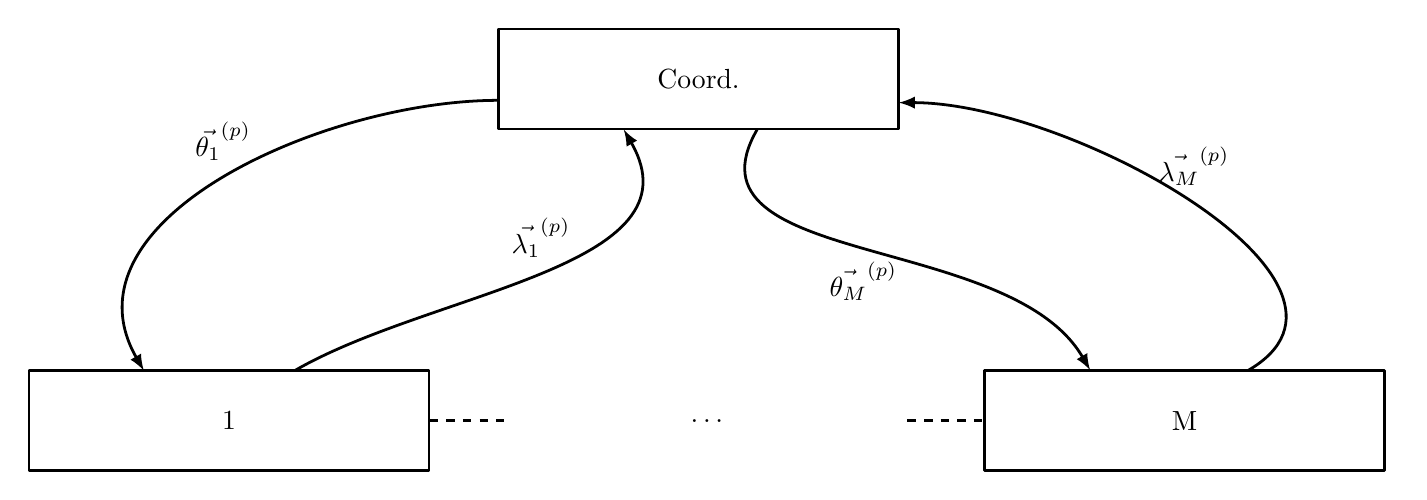
\begin{tikzpicture}[>=latex,line join=bevel,]
      \pgfsetlinewidth{1bp}
      %% 
      \begin{scope}
        \pgfsetstrokecolor{black}
        \definecolor{strokecol}{rgb}{1.0,1.0,1.0};
        \pgfsetstrokecolor{strokecol}
        \definecolor{fillcol}{rgb}{1.0,1.0,1.0};
        \pgfsetfillcolor{fillcol}
      \end{scope}
      \pgfsetcolor{black}
      % Edge: a_1 -> a_3
      \draw [->] (262.09bp,122.8bp) to[out=-120,in=120] node[below=0.02cm] {$\vec{\theta_M}^{(p)}$} (381.97bp,36.225bp);
      % Edge: a_3 -> a_1
      \draw [->] (438.82bp,36.094bp) to[out=30,in=0] node[above=0.1cm] {$\vec{\lambda_M}^{(p)}$} (313.09bp,132.52bp);
      % Edge: a_2 -> a_1
      \draw [->] (95.811bp,36.138bp) to[out=30,in=-60] node[above=0.05cm] {$\vec{\lambda_1}^{(p)}$} (214.09bp,122.79bp);
      % Edge: a_4 -> a_3
      \draw [dashed] (316.23bp,18.0bp) .. controls (325.45bp,18.0bp) and (334.67bp,18.0bp)  .. (343.9bp,18.0bp);
      % Edge: a_1 -> a_2
      \draw [->] (168.84bp,133.34bp) to[out=180,in=120] node[above=0.1cm] {$\vec{\theta_1}^{(p)}$} (41.325bp,36.047bp);
      % Edge: a_2 -> a_4
      \draw [dashed] (144.23bp,18.0bp) .. controls (153.45bp,18.0bp) and (162.67bp,18.0bp)  .. (171.9bp,18.0bp);
      % Node: a_4
      \begin{scope}
        \definecolor{strokecol}{rgb}{0.0,0.0,0.0};
        \pgfsetstrokecolor{strokecol}
        \draw (244.0bp,18.0bp) node {$\dots$};
      \end{scope}
      % Node: a_3
      \begin{scope}
        \definecolor{strokecol}{rgb}{0.0,0.0,0.0};
        \pgfsetstrokecolor{strokecol}
        \draw (488.0bp,36.0bp) -- (344.0bp,36.0bp) -- (344.0bp,0.0bp) -- (488.0bp,0.0bp) -- cycle;
        \draw (416.0bp,18.0bp) node {M};
      \end{scope}
      % Node: a_2
      \begin{scope}
        \definecolor{strokecol}{rgb}{0.0,0.0,0.0};
        \pgfsetstrokecolor{strokecol}
        \draw (144.0bp,36.0bp) -- (0.0bp,36.0bp) -- (0.0bp,0.0bp) -- (144.0bp,0.0bp) -- cycle;
        \draw (72.0bp,18.0bp) node {1};
      \end{scope}
      % Node: a_1
      \begin{scope}
        \definecolor{strokecol}{rgb}{0.0,0.0,0.0};
        \pgfsetstrokecolor{strokecol}
        \draw (313.0bp,159.0bp) -- (169.0bp,159.0bp) -- (169.0bp,123.0bp) -- (313.0bp,123.0bp) -- cycle;
        \draw (241.0bp,141.0bp) node {Coord.};
      \end{scope}
      % 
    \end{tikzpicture}
  }
  \caption[Primal decomposition-based \dmpc{}.]{Primal decomposition-based \dmpc{}. \todo{remake figure}}\label{fig:dmpc_communication}
\end{figure}
\begin{remark}
  The same decomposition can be used if the coupling constraints are equalities or if there are local constraints for the subsystems.
  We can change problems~\eqref{eq:DOP_local} and~\eqref{eq:projectedSubgradient_lambda} accordingly to respect such modifications, i.e.\ adding the local constraints to the local problems and changing the inequality constraints to equality ones, including in the set $\set{S}$.
  An example is given in the next section.
\end{remark}

\section{Example and Interpretations}\label{sec:example-interpr}
As a simple numerical example to illustrate the functioning of the algorithm we take two \mbox{$1$-dimensional} \siso{} systems coupled by the inputs ($M=2$,$n_{x}=1$,$n_{c}=1$).
The systems have no physical meaning but due to their small scale it is easier to visualize.

The systems are described by the following \ltidt{} dynamics
\begin{equation}
  \label{eq:example_dynamics}
  x_{i}[k+1]=a_{i}x_{i}[k]+b_{i}u_{i}[k]
\end{equation}
with $a_{1}=0.8$, $a_{2}=0.6$, $b_{1}=0.3$, $b_{2}=0.4$, and
constraint by an equality constraint
\begin{equation}
  \label{eq:example_equality}
  u_{1}+u_{2}=\vec{u}_{\max}
\end{equation}
with $\vec{u}_{\max}=4$.
We use a \dmpc{} with horizon ${\predhorz=2}$ and references and gains that results in the problems
\begin{equation}
  \begin{matrix}
    \underset{\vec{U}_{i}[k]}{\mathrm{minimize}}&\obji=\frac{1}{2}\norm{\vec{U}_{i}[k]}^{2}_{H_{i}} + {\vec{f}_{i}[k]}^{T}\vec{U}_{i}[k]\\
    \mathrm{subject~ to} & \bar{\Gamma}_{i}\vec{U}_{i}[k] = \thetaik:\lambdaik
  \end{matrix}
  \label{eq:example_local_problem}
\end{equation}
with
\begin{equation}
  \label{eq:1}
  \begin{array}{ccc}
    H_1=\left(\begin{array}{cc} 1.9446 & 0.4608\\ 0.4608 & 1.5760 \end{array}\right),
                                                         &
    \vec{f}_1[k]=\left(\begin{array}{c} -6.6624\\ -4.1280 \end{array}\right),
                                       &
     \bar{\Gamma}_{1}= I_{2},
    \\
    \\
    H_2=\left(\begin{array}{cc} 1.7834 & 0.3456\\ 0.3456 & 1.5760 \end{array}\right),
                                                         &
    \vec{f}_2[k]=\left(\begin{array}{c} -7.6032\\ -5.4720 \end{array}\right),
    &
    \bar{\Gamma}_{2}=I_{2}.
  \end{array}
\end{equation}
The coordinator update function
\begin{equation}
\vec{\theta}[k]\pplusone=\Proj^{\set{S}}(\vec{\theta}[k]\p+\rho\p\vec{\lambda}[k]\p),
\end{equation}
with ${\set{S} = \setbuild{\vec{\theta}[k]}{I_{c}^{M}\vec{\theta}[k] = \vec{u}_{\max}}}$, $c=n_{u}\predhorz=2$.

From now on, we remove the $[k]$ indices for convenience, since all calculation is valid for the same step $k$ unless expressly stated otherwise.

This euclidean projection can be calculated explicitly yielding
\begin{equation}
    \vec{\theta}\pplusone=\vec{\theta}\p-\rho\p\vec{\lambda}\p-{I_{c}^M}/({I_{c}^M}\T {I_{c}^M})\left({I_{c}^M}\T(\vec{\theta}\p-\rho\p\vec{\lambda}\p) -\vec{u}_{\max}\right).
\end{equation}

If the initial ${\vec{\theta}}^{(0)}$ belongs to $\set{S}$, we can rewrite for each individual $\thetai$:
\begin{equation}
  \label{eq:example_projectedSubgradient_lambda}
 \thetai\pplusone=\thetai\p+\rho\p\left(\lambdai\p-\frac{1}{M}\sum_{j=1}^{M}\vec{\lambda}_j\p\right),\forall i\in\set{M}
\end{equation}

Using~\eqref{eq:example_local_problem} and~\eqref{eq:example_projectedSubgradient_lambda} with initial conditions ${x_{1}[0]=2}$ and ${x_{2}[0]=2}$, and state references ${w_{1}[0]=1.5x_{1}[0]}$ and ${w_{2}[0]=1.5x_{2}[0]}$, we can program Algorithm~\ref{alg:primal_decomposition_based_dmpc}.
The dynamics of variables $\vec{\theta}_{i}[0]$ $\vec{\lambda}_{i}[0]$ during the iterative process can be seen in Figs.~\ref{fig:example_theta} and~\ref{fig:example_lambda}.

\begin{figure}[h]
  \centering
  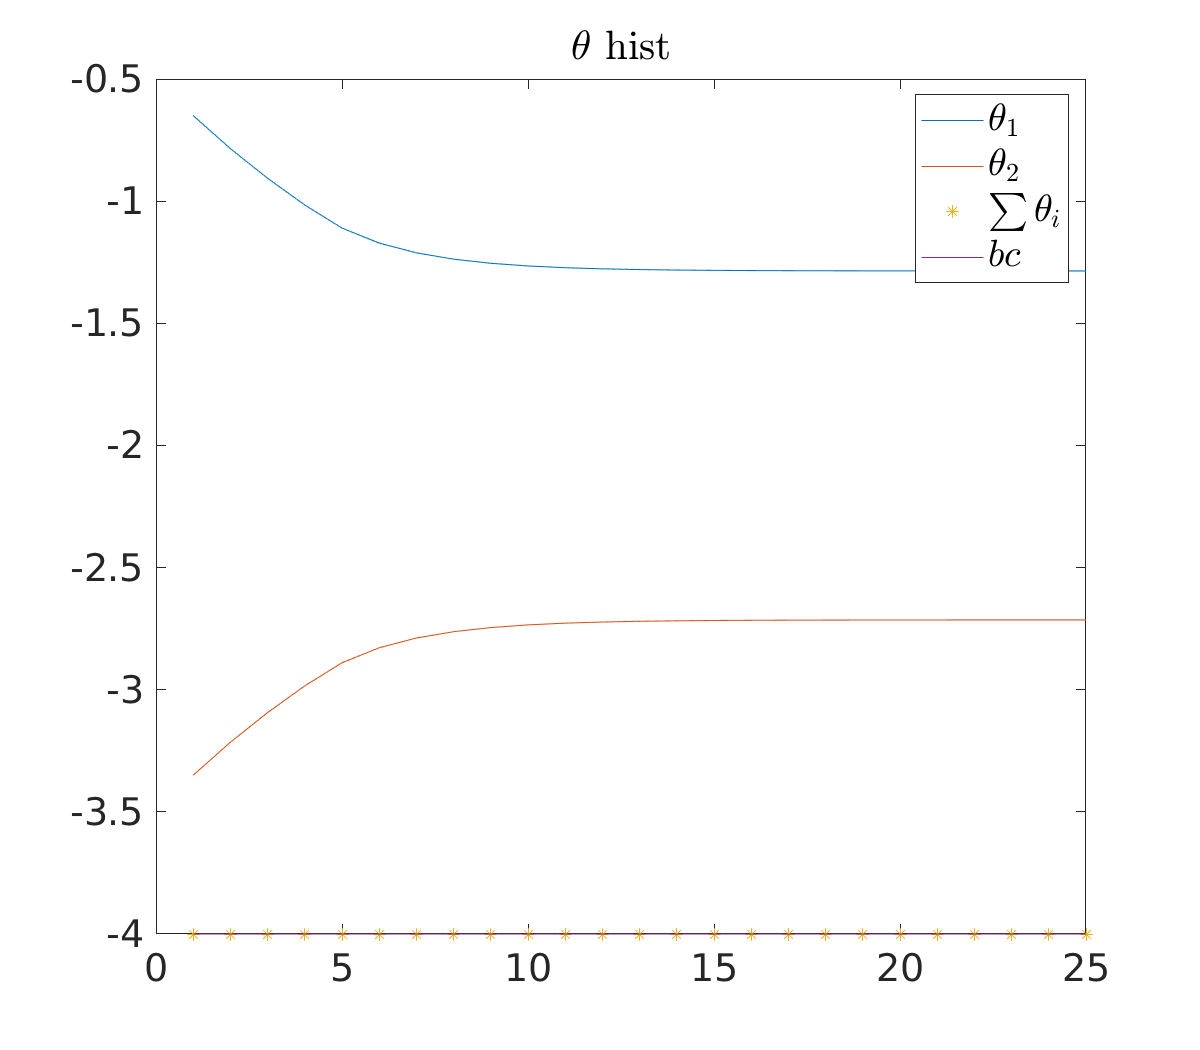
\includegraphics[width=.5\textwidth]{../img/example_theta.png}
  \caption{Evolution of $\thetai$ during iterative process. \todo{remake figure}}\label{fig:example_theta}
\end{figure}

\begin{figure}[h]
  \centering
  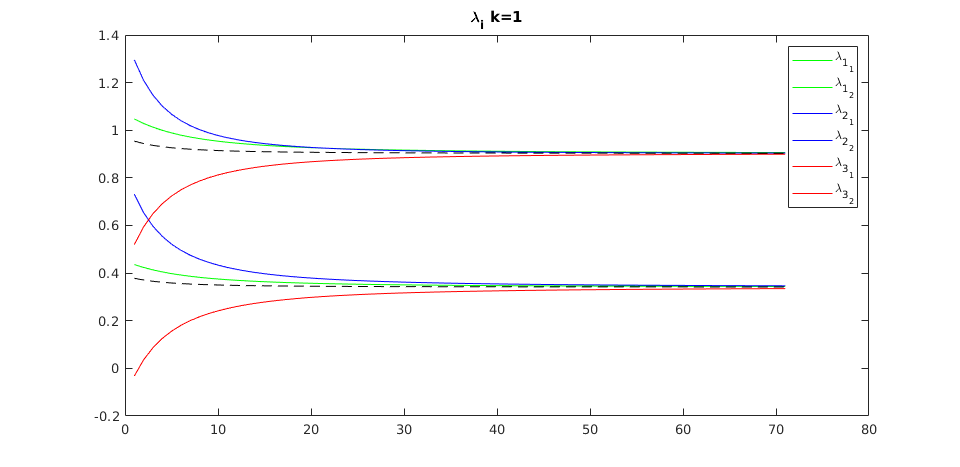
\includegraphics[width=.5\textwidth]{../img/example_lambda.png}
  \caption{Evolution of $\lambdai$ during iterative process. \todo{remake figure}}\label{fig:example_lambda}
\end{figure}
In Figs.~\ref{fig:example_theta} and~\ref{fig:example_lambda} the sub-systems were color coded in nuances of \todo{blue} for agent $1$ and nuances of \todo{green} for agent $2$.
Observe in Fig.~\ref{fig:example_theta} that the agent with the bigger values of $\thetai$ has a corresponding $\lambdai$ smaller than the other agent.
In next iterations the bigger $\thetai$ decrease and the smaller ones increase, until they stabilize.

For $\lambdai$ we see it stabilizes exactly in the middle of the initial values.
It is true due to the global equality constraint whose simple projection onto the intersection of hyperplanes result in~\eqref{eq:example_projectedSubgradient_lambda}.
Moreover, as one can see, the iterative process converges if ${\thetai\pplusone=\thetai\p}$, which happens when ${\lambdai\p=\frac{1}{M}\sum_{j=1}^{M}\vec{\lambda}_j\p}$.
Although it is not necessarily true for the inequality cases it can gives an insight of the functioning of the algorithm.
The values of $\thetai$ can represent an allocation of the maximum input given to the agents by the coordinator, and $\lambdai$ as a measure of dissatisfaction of each agent to the value allocated.
So the coordinator has as role to negotiate the values of the allocations so all agents can be equally dissatisfied.
Due to this process of iterative allocations, other names given for this decomposition are \textbf{resource allocation} and \textbf{quantity decomposition}.

We can create a parallel with the cake-cutting problem~\cite{BramsTaylor1995} where two (or more) agents want to share a cake dividing it equally so no agent envy the piece of cake of other agent.
Usually in these kinds of problems, a protocol is created where agents cut successively the cake and the other agents take parts which they think it is the greater.
But in those cases usually all agents have the same hunger.

In our case, agents may have different needs (represented by the matrices $\bar{\Gamma}_{i}$).
So the coordinator works as a mediator positioning the cake cutter, showing where it would cut the cake ($\thetai$ during the iterative process) and asks if the agents would be satisfied ($\lambdai$) and adjust the cake cutter until a consensus is reached. Due to this interpretation we call the iterative process as a \textbf{negotiation phase}.

% \begin{remark}
%   Observe that in this decomposition \textbf{``Liar'' agent attacks} as in \cite{VelardeEtAl2017b} cannot happen, since the input constraint is given by the coordinator.
% \end{remark}

% \begin{description}
%   \item[Show examples of Attacks]
%   \item[False data injection/communication corruption] \todo{show that since coordinator is oblivious to what happen inside each agent what matters is what it receives, no need to specify exactly the responsible part which generated attack}
% \end{description}
% but they will always reflect on the channel.
% \begin{description}
%   \item[Negotiation Stability] Show example and how cheating can destabilize negotiation
%         \begin{enumerate}
%           \item Analysis of eigenvalues of negotiation
%         \end{enumerate}
%   \item[Example of how attacker can drive negotiation to other points]
% \end{description}
% \begin{figure}[h]
%   \centering
%   \begin{subfigure}{.45\textwidth}
%     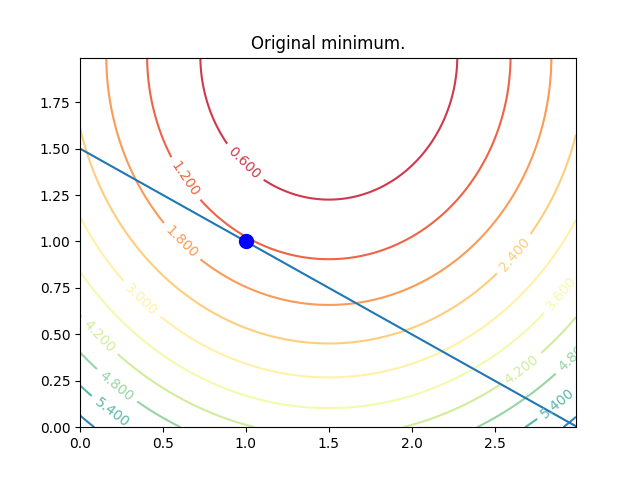
\includegraphics[width=\textwidth]{../img/original-minimum.png}
%     \caption{Original minimum.}
%     \label{fig:first}
%   \end{subfigure}
%   \hfill
%   \begin{subfigure}{0.45\textwidth}
%     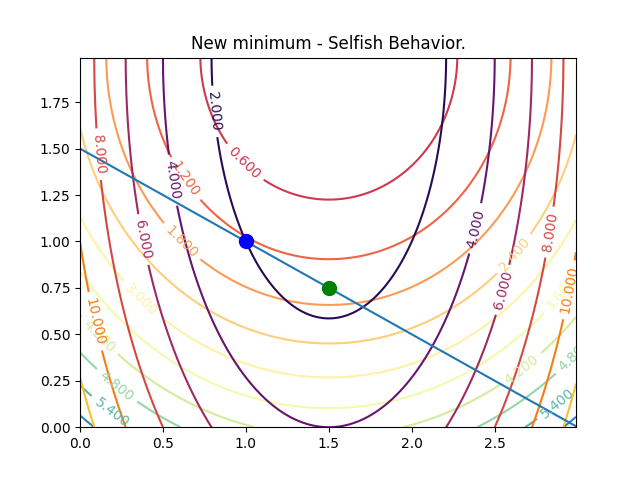
\includegraphics[width=\textwidth]{../img/new-minimum-selfish.png}
%     \caption{Minimum after non-conforming behavior.}
%     \label{fig:second}
%   \end{subfigure}
%   \caption{Effects of non-conforming behaviors on optimal value. \todo{Refaire les images}}
%   \label{fig:figures}
% \end{figure}

% General discussion about ways to secure negotiation, here we discuss what
% \begin{description}
%   \item[Discussion about Methods]
%   \item[Discussion about Detection and Isolation]
%         \begin{description}
%           \item[Learning methods] Use input labeled data to train detector
%           \item[Analytical methods] Use model of the system and residuals
%         \end{description}
%   \item[Discussion about Recovery] Could show different cases
%         \begin{description}
%           \item[Active methods] Need detection
%           \item[Passive methods] Robust control
%         \end{description}
% \end{description}


% \begin{figure}[h]
%   \centering
%   \begin{subfigure}{0.45\textwidth}
%     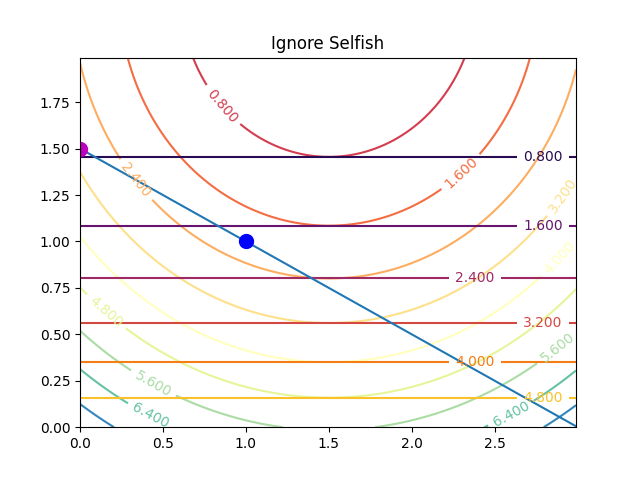
\includegraphics[width=\textwidth]{../img/ignoreX.png}
%     \caption{Optimal value after ignoring attacker.}
%     \label{fig:third}
%   \end{subfigure}
%   \hfill
%   \begin{subfigure}{0.45\textwidth}
%     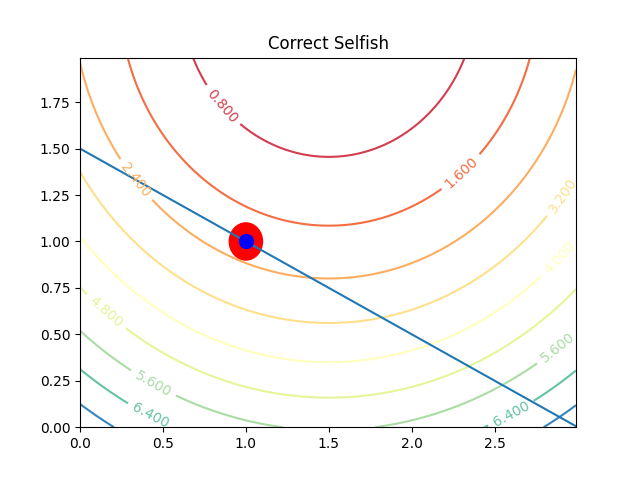
\includegraphics[width=\textwidth]{../img/correctX.png}
%     \caption{Optimal value after trying to recover original behavior.}
%     \label{fig:third}
%   \end{subfigure}

%   \caption{Recovering options.}
%   \label{fig:figures}
% \end{figure}


% Model 3R-2C \cite{GoudaEtAl2002}
% \begin{figure}[h]
%   \centering
%   \begin{circuitikz}[european]
%     \draw (0,0) node[tlground]{} to[isource, l=$P^{\text{heat}}$] ++(0,2) to[short, -*] ++(1.5,0) coordinate (a);

%     \draw (a) node[above]{$T^{\text{in}}$}  to[C=$C^{\text{air}}$] ++(0,-2) node[tlground]{};
%     \draw (0,-3) node[tlground]{} to[isource, l=$I^{\text{sol}}$] ++(0,2)
%     to[short, -*] ++(1.5,0) coordinate (b);
%     \draw (b) to[C=$C^{\text{walls}}$] ++(0,-2) node[tlground]{};

%     \draw (a) -- ++(2,0) coordinate (c) -- ++(0,-.5) to[R=$R^{\text{iw/ia}}$] ++(0,-2) -- ++(0,-.5) coordinate (d);

%     \draw (b) node[above]{$T^{\text{walls}}$} to[short,-*] (d);

%     \draw (c) --  ++(2.5,0) -- ++(0,-.5) to[R=$R^{\text{oa/ia}}$] ++(0,-2) -- ++(0,-.5) coordinate (e);

%     \draw (d) to[R=$R^{\text{ow/oa}}$] (e) to[battery,l=$T^{\text{out}}$] ++(0,-2) node[tlground]{};
%   \end{circuitikz}
%   \caption{Thermic Model 3R-2C of a room.}
%   \label{fig:3R2C_model}
% \end{figure}

% The state-space model of each subsystem is given by:
% \begin{equation}
%   \begin{matrix}
%     \label{eq:systems_cont}
%     \dot{\vec{x}}_{i}(t)  &=&{A_{c}}_{i}\vec{x}_{i}(t) &+& {B_{c}}_{i}\vec{u}_{i}(t)\\
%     \vec{y}_{i}(t)        &=&{C_{c}}_{i}\vec{x}_{i}(t) &&
%   \end{matrix},
% \end{equation}
% where
% \begin{equation}
%   \label{eq:4}
%   \begin{matrix}
%     A_{\mathrm{c}_{i}}=\left[
%       \begin{matrix}
%         -\frac{1}{C^{\text{walls}}_{i}R^{\text{oa/ia}}_{i}}-\frac{1}{C^{\text{walls}}_{i}R^{\text{iw/ia}}_{i}}& \frac{1}{C^{\text{walls}}_{i}R^{\text{iw/ia}}_{i}}\\
%         \frac{1}{C^{\text{air}}_{i}R^{\text{iw/ia}}_{i}} &-\frac{1}{C^{\text{air}}_{i}R^{\text{ow/oa}}o_{i}}-\frac{1}{C^{\text{air}}_{i}R^{\text{iw/ia}}_{i}}
%       \end{matrix}\right]\\
%     \begin{matrix}
%       B_{\mathrm{c}_{i}}=\left[
%         \begin{matrix}  \frac{10}{C^{\text{walls}}_{i}}& 0\end{matrix}
%       \right]\T&C_{\mathrm{c}_{i}}=\left[\begin{matrix}1 & 0\end{matrix}\right]
%     \end{matrix}
%   \end{matrix}
% \end{equation}
% where ${\vec{x}_{i}=[{{x}_{A}}_{i}\T\ {{x}_{W}}_{i}\T]\T}$. ${x_A}_i$ and ${x_W}_i$ are the mean temperatures of the air and walls inside room~$i$. $\vec{u}_{i}$ is the input (the heating power)
% for the corresponding room. The inputs are constraint by ${\sum_{i=1}^{4}\vec{u}_{i}(t)\preceq 4\mathrm{kW}}$.

% \begin{table}[b]
%   \centering
%   \caption{Model Parameters}\label{tab:modelParamMeaning}
%   \begin{tabular}[b]{cl}
%     \toprule
%     Symbol&Meaning\\
%     \midrule
%     $C^{\text{air}}_{i}$  &Heat Capacity of Inside Air\\
%     $C^{\text{walls}}_{i}$ &Heat Capacity of External Walls\\
%     $R^{\text{iw/ia}}_{i}$ &Resist. Between Inside Air and Inside Walls\\
%     $R^{\text{ow/oa}}_{i}$ &Resist. Between Outside Air and Outside Walls\\
%     $R^{\text{oa/ia}}_{i}$ &Resist. Between Inside and Out.\ Air (from windows)\\
%     \bottomrule
%   \end{tabular}
% \end{table}

% \begin{table}[b]
%   \centering
%   \caption{
%     Parameters for each agent}\label{tab:modelParam}
%   \begin{tabular}[t]{cccccc} \toprule
%     Symbol& I & II & III & IV &Unit\\
%     \midrule
%     $C^{\text{walls}}$   &$5.4$&$4.9$&$4.7$&$4.7$ &$10^{4}\mathrm{J/K}$ \\
%     $C^{\text{air}}$     &$7.5$ &$8.4 $&$8.2$ &$7.7$&$10^{4}\mathrm{J/K}$  \\
%     $R^{\text{oa/ia}}$   &$5.2$&$4.6$&$4.9$&$5.4$&$10^{-3}\mathrm{K/W}$ \\
%     $R^{\text{iw/ia}}$   &$2.3$&$2.4$&$2.3$&$2.9$&$10^{-4}\mathrm{K/W}$\\
%     $R^{\text{ow/oa}}$   &$1.5$&$0.6$&$0.7$&$0.7$& $10^{-4}\mathrm{K/W}$ \\
%     \bottomrule
%   \end{tabular}
% \end{table}

\end{document}
